\section{Describing Variation of Time-Dependent Output}\label{sec:sa_time_dependent_variation}

Ramsay and Silverman \cite{Ramsay2005} popularized \gls{fda}, which refers to statistical analyses of data that are functions.
The main assumption of \gls{fda}, as opposed to a more conventional multivariate analysis, is that data present sufficient smoothness, defined by existence of derivatives up to a certain order.
Another distinguishing feature of \gls{fda}, as opposed to time-series analysis or spatial statistics, is the availability of numerous replications of such data (i.e., set of functions) produced by the same or similar underlying process. 
The goal of \gls{fda} related to this work is to describe the overall variation of a set of functions using a smaller set of scalars.
These scalars, in turn, can be used as the \gls{qoi} for \gls{sa}.

\subsection{Functional Output Representation}\label{sub:sa_spline}

The assumption of continuity within a practically discrete data set (such as the numerical code output of Eq.~(\ref{eq:discrete_time}) is made explicit through a functional representation.
The recommended representation is through a linear combinations of basis functions \cite{Ramsay2005}.
This thesis adopts the B-spline basis function \cite{Gillies2010} expansion because of its flexibility \cite{Eilers1996,Eilers2010} 
and the wide availability of its implementation in open numerical libraries \cite{RCT2017}.

Within this framework, a function can be written using basis function expansion as,
\begin{equation}
	y_i (t) = \sum_{k = 1}^{K} c_{ik} \cdot \phi_k (t); \quad i = 1, 2, \cdots N
\label{eq:basis_function_expansion}
\end{equation}
where $K$ indicates the number of basis functions. $\phi_k (t)$ is the $k$-th basis function, 
and $c_{ik}$ is the basis coefficient.
The latter is fitted to the data set to construct curve $i$ with or without smoothing (i.e., interpolating condition vs. penalized ).

A B-spline basis function is a basis system constructed using piecewise polynomial (\emph{spline}) connected at select points in the domain called \emph{knots}.
Let $\boldsymbol{\tau}=\{\tau_l; l = 0,1,\cdots, L\}$ be a sequence of knots, non-decreasing numbers that divide the function domain into $L$ sub-intervals.
Within each of these sub-intervals, piecewise polynomial of degree $p$ is defined.
At the interconnection, adjacent polynomials are continuous with derivatives up to $p-1$ match up.

The basis functions in the B-spline system are determined by the degree of the polynomial $p$ and the knot sequence sequence $\boldsymbol{\tau}=\{\tau_l; l = 0,1,\cdots, L\}$.
At the left and right boundaries, several spline basis functions are defined with decreasing continuity up to being discontinuous in the either end.
To satisfy these condition, the endpoints are repeated and augmented into the knot sequence such that
\begin{equation}
	\tau_{-(p-2)} = \cdots = \tau_{0} \leq \tau_{1} \leq \cdots \leq \tau_{L} = \cdots = \tau_{L+(p-2)} 
\label{eq:augmented_knots}
\end{equation}
As such, the augmented knot becomes $\boldsymbol{\tau}=\{\tau_l; l = 0,1,\cdots, L + 2p\}$.
B-spline basis functions of degree $p$ can then be defined recursively on the augmented knot sequence using de Boor - Cox formula as follows, 
\begin{equation}
	\begin{split}
		B^0_k = 
			\begin{cases}
				1, & \tau_k \leq t < \tau_{k+1} \\
			0, & \text{otherwise}
	\end{cases} \\
	B^p_k =  \alpha^p_k (t) B^{p-1}_k + \left[1 - \alpha^p_{k+1} (t)\right] B^{p-1}_{k+1} \\
	\alpha^p_k (t) =
	\begin{cases}
				\frac{t - \tau_i}{\tau_{i+p}-\tau_i}, & \tau_{i+p} \neq \tau_i \\
			  0, & \text{otherwise}
	\end{cases}
	\end{split} 
\label{eq:}
\end{equation}
where $B_k^p (t)$ denotes the $k$-th B-spline of degree $p$.
The degree, $p$, and the number of interior knots, $L-1$, (that is excluding the end points) determine the number of spline basis functions according to $K = p + L$.

Fig.~\ref{fig:b_spline} illustrates all the fourteen spline basis functions of degree $3$ over $10$ uniform interior knots defined in $[0,1]$.
The three leftmost and three rightmost basis functions are less smooth compared to the other (twice continuously differentiable) eight basis functions in the center. 
From leftmost to the right (rightmost to the left) the basis functions are discontinuous, continuous, and once continuously differentiable at the left (right) boundaries, respectively.
\begin{figure}[bth]
	\centering
	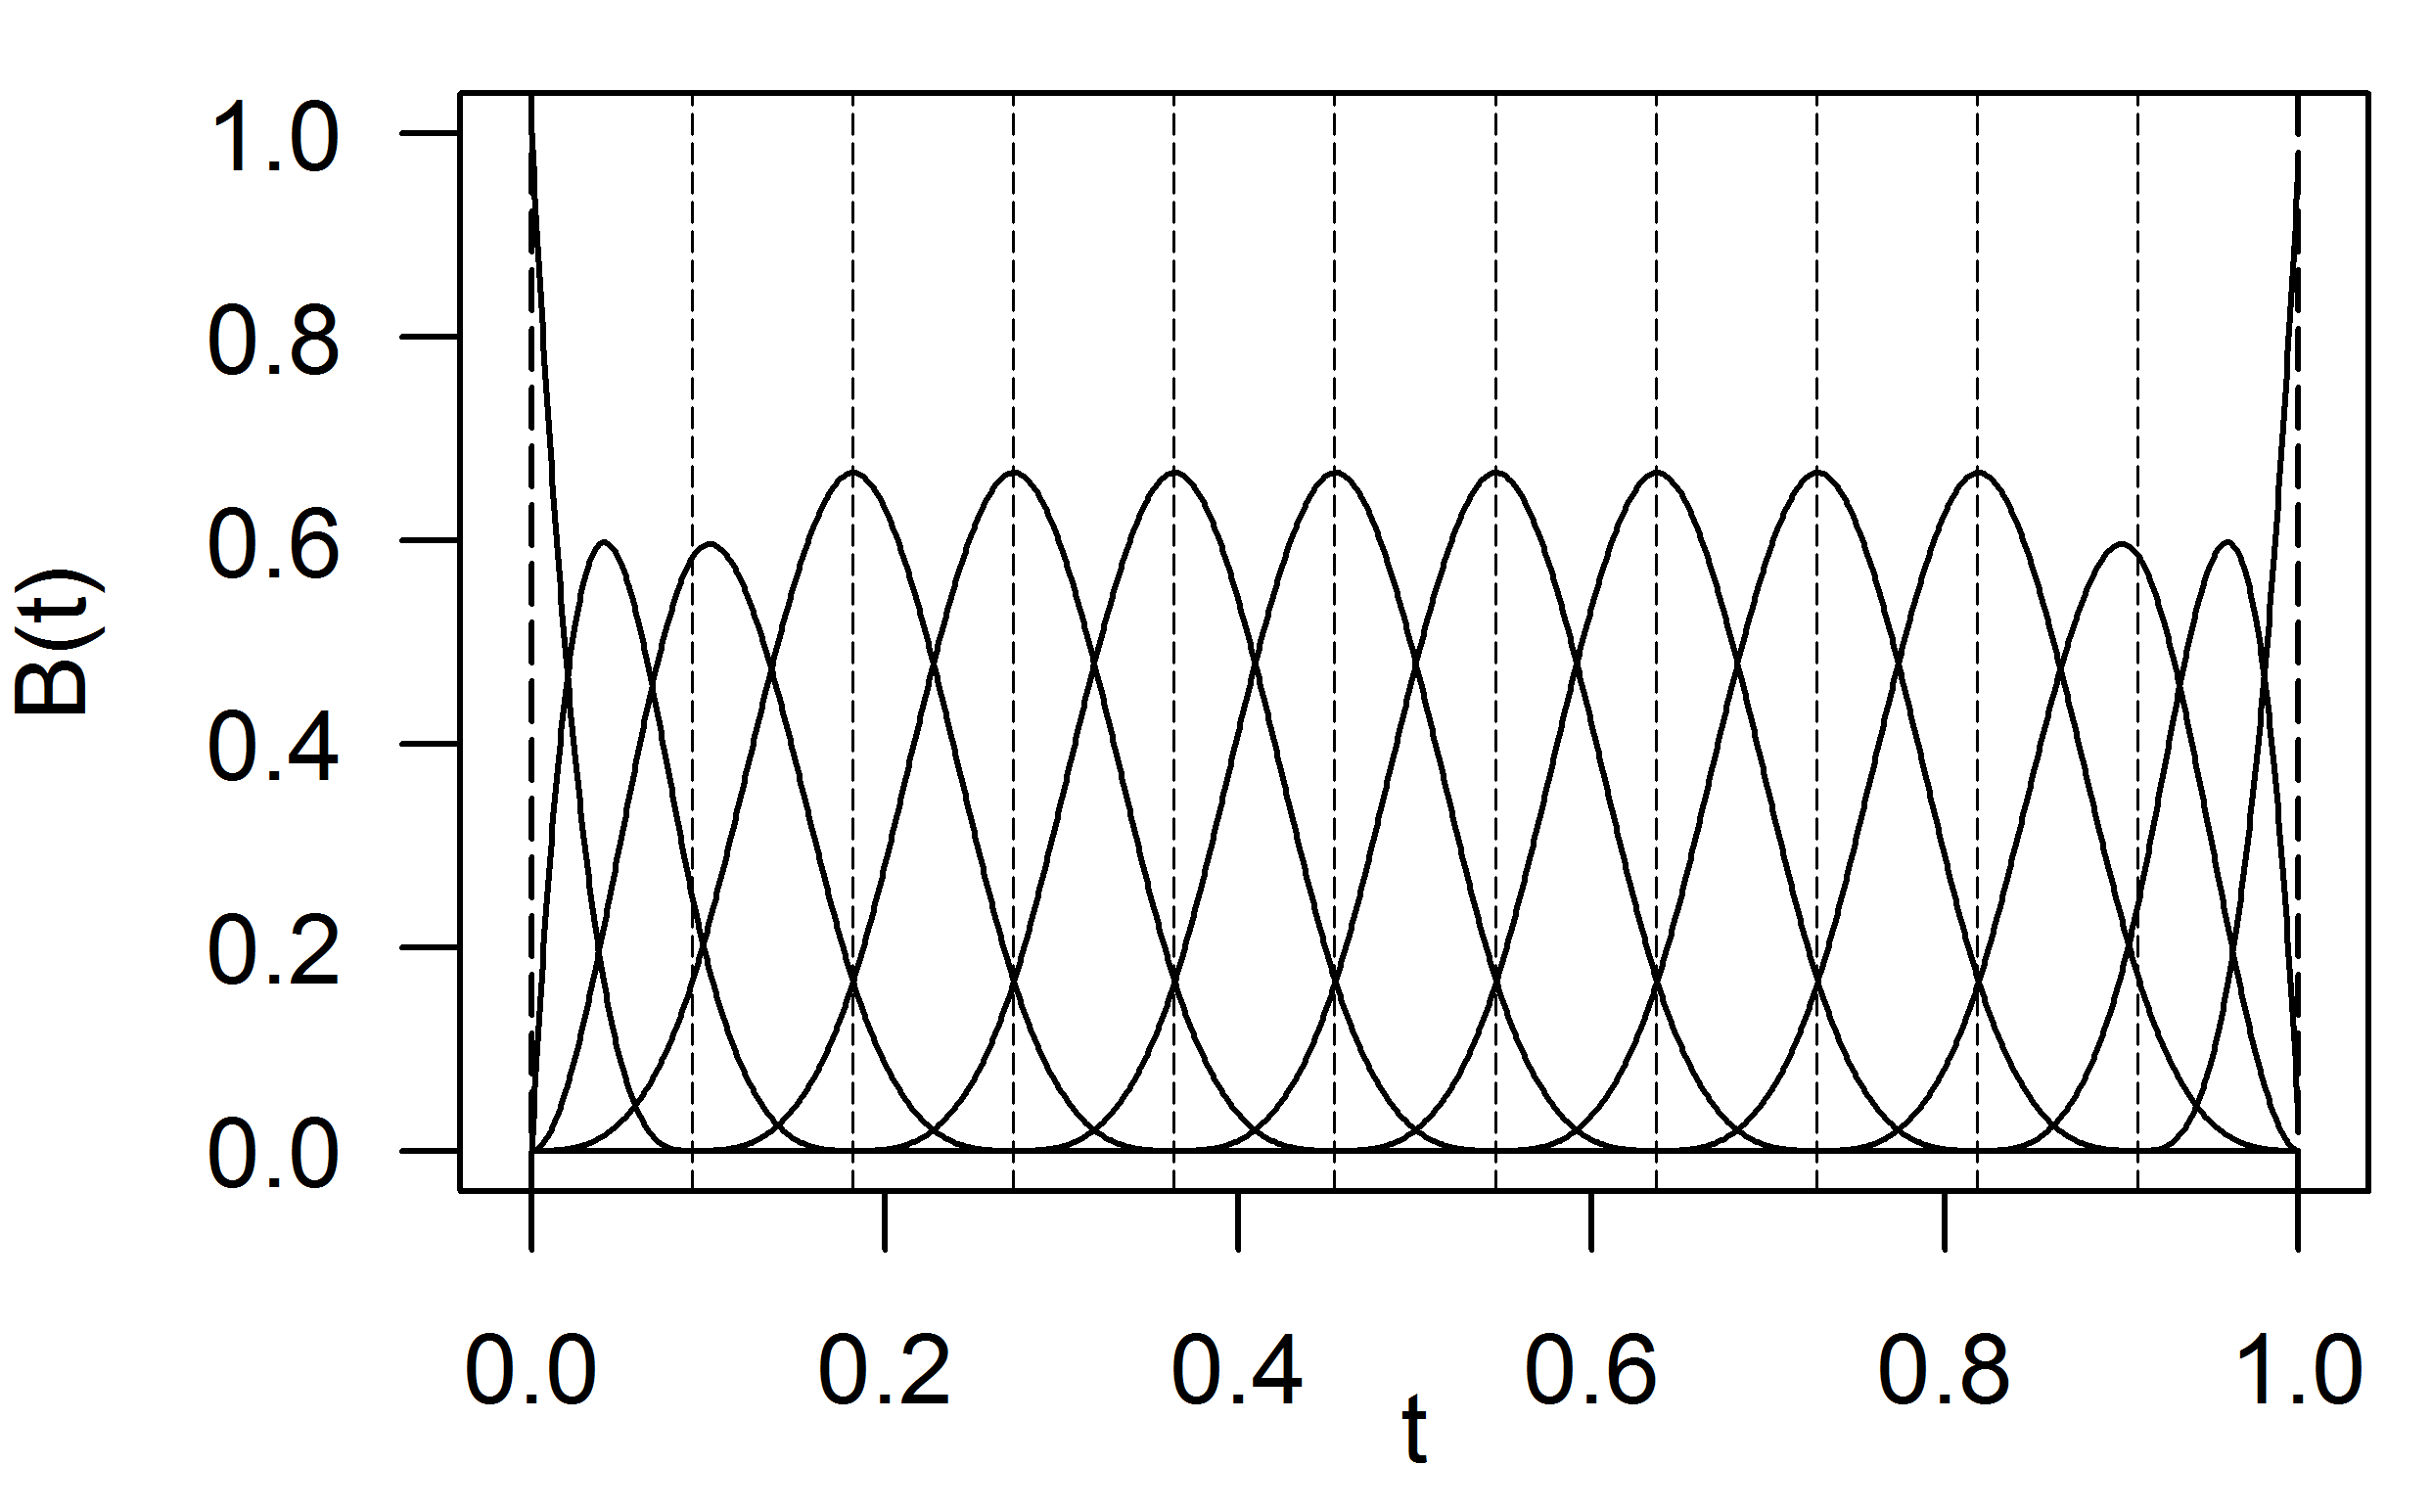
\includegraphics[width=1.0\textwidth]{../figures/r-figures/bSpline.png}
	\caption[Spline basis functions of order $4$]{The fourteen spline basis functions of degree $3$ (cubic) with $10$ uniform interior knots (shown in light dashed vertical lines) that divides the domain into 11 sub-intervals}
	\label{fig:b_spline}
\end{figure}

\subsection{Curve Registration by Landmarks}\label{sub:sa_registration}

Two types of variations are often simultaneously present in a functional dataset: the variation in magnitude (\emph{vertical} variation) and the variation in phase (\emph{horizontal} variation).
The simultaneous presence of these two types of variations makes even the definition of a mean function difficult \cite{Kneip1992}. (see illustration)
To address this issue, the two types of variation are first separated through a registration procedure.
The procedure transforms the time argument using a warping function such that there is less phase variation in the dataset.
In this work, the landmark type registration type is employed because the main features of the function of interest (i.e., reflood curve) are readily identifiable.
In a functional data set with phase variation, this particular type of registration forces important events in a curve (its \emph{landmarks}) to occur at the same time.

\subsection{Functional Principal Component Analysis}\label{sub:sa_fpca}

Separation of phase variation from magnitude variation by registration procedure allows for the definition of a proper mean function.
With respect to that, the notion of functional variation can be defined.
The covariance function of a set of function realizations $\{y_n(t);n = 1, 2, \cdots, N; t \in [t_a,t_b]\}$ from a random process $Y$ is defined as
\begin{equation}
	\nu (t_1, t_2) \equiv \frac{1}{N} \sum_{n=1}^{N} (y_n(t_1) - \bar{y}(t_1)) \cdot (y_n(t_2) - \bar{y}(t_2))
\label{eq:covariance_function}
\end{equation}

To extract more meaningful information from the covariance function, the function is often projected onto lower-dimensional space using an orthogonal decomposition.
This projection can be done through the functional principal component (fPC) analysis (fPCA) (also know as the Karhunen-Lo\'eve transform):
\begin{equation}
	\nu (t_1, t_2) = \sum_{j=1}^{+\infty} \rho_j \cdot \xi_j(t_1) \cdot \xi_j(t_2)
\label{eq:kl_transform}
\end{equation}
where $\rho_j$ is a series of ordered eigenvalues of decreasing values; 
$\xi_j(t)$ is the corresponding series of orthogonal eigenfunctions (or the fPC).

The transformation of the covariance function into pairs of eigenvalues and eigenfunctions also allows each element of the original dataset $\{y_n(t)\}$ to be represented as a series that is optimal in the root-mean-square-of-error sense:
\begin{equation}
  y_n(t) = \bar{y}(t) + \sum_{j=1}^{+\infty} \theta_{j,n} \cdot \xi_j (t); \quad n = 1, 2, \cdots, N
\label{eq:pod}
\end{equation}
were the fPC score $\theta_{j,n}$ associated with each realized function is defined by the orthogonality condition
\begin{equation}
  \theta_{j,n} = \int_(t_a)^(t_b) \left[y_n(t) - \bar{y}(y)\right] \cdot \xi_j (t) dt
\label{eq:pod_orthogonality}
\end{equation}

Eqs.~(\ref{eq:pod}) and (\ref{eq:pod_orthogonality}) imply that across realizations in the samples, 
$\{y_n(t)\}$ can represented linearly using a common mean function and sums of deviation terms from the mean.
The deviation terms consist of a set of common eigenfunctions and a set of fPC scores.
As such, the random character of each realization is left to the score associated with each component and each realization.
Put differently, the eigenfunctions described the (common) modes of variations, 
while the scores quantify the strength of a particular mode~\cite{Wang2012}.
These scores will be used as the \gls{qoi} in the subsequent global \gls{sa}. 